\subsection{Field Cage for protoDUNE Dual Phase}~\label{sec:proto-dune-dp-fc}
Field cages provide uniform electric fields for ionization electrons to drift to anodes for the detection in the Time Projection Chamber. The baseline design for DUNE LArTPC is that of the single phase in which the ionization electrons created by the secondary particles resulting in neutrino-nucleon interactions drift in LAr and get detected on the anode plane that resides inside the liquid phase of argon. An alternative design is the dual phase design in which the ionization electrons drift vertically and then be extracted in the gas phase via a large aread electron multiplier (LEM). The DUNE baseline design technology is single phase, however, the dual phase detector provides a complementary technology with a potentially lower energy threshold and pixelated readout which eliminates degeneracies associated with wire based readout.

During P.I. Yu's sabbatical at CERN he began work with the WA105 $1m\times 1m\times 3m$ prototype. This work provided the opportunity for Yu to join the WA105 collaboration and begin work on the larger $6m\times 6m\times 6m$ prototype as the first U.S. collaborating institution. The large scale dual phase technology is still in the R$\&$D phase with many technological challenges to be faced and thus is currently a lower priority compared to the single phase LArTPC effort. However, U.S. participation in this effort is benificial to aiding in the development of the dual phase detector as well as strengthening the international nature of DUNE collaboration, an essential ingredient in its success.

UTA hopes to play a lead role in the in the design and construction of the protoDUNE experiments and thus allow us to gain the expertise to contribute to the construction of the first DUNE far detector module in the early 2020's. The dual phase field cage (FC) is an example of a component of the dual phase and single phase detector where common aspects of the detector design and construction can be found. P.I. Yu, with input from DUNE management, has agreed to take responsibility for the design and construction of the dual phase field cage in collaboration with the University of Zurich, CERN, and Fermilab.


Figure~\ref{fig:if-dp-fc} shows the current conceptual design of the FC for the DP protoDUNE experiment.  The concept is to use a compartmentalized structure of submodules that consist of several straight profiles to provide voltage differentials for the generation of a uniform drift field in the bulk liquid argon. The use of straight profiles made of either aluminum or stainless steel makes the pre-assembly and shipment of submodules convenient. Each of these submodules will be designed to hold voltage of 300kV for the dual phase.

\begin{figure}[htb]
\centering
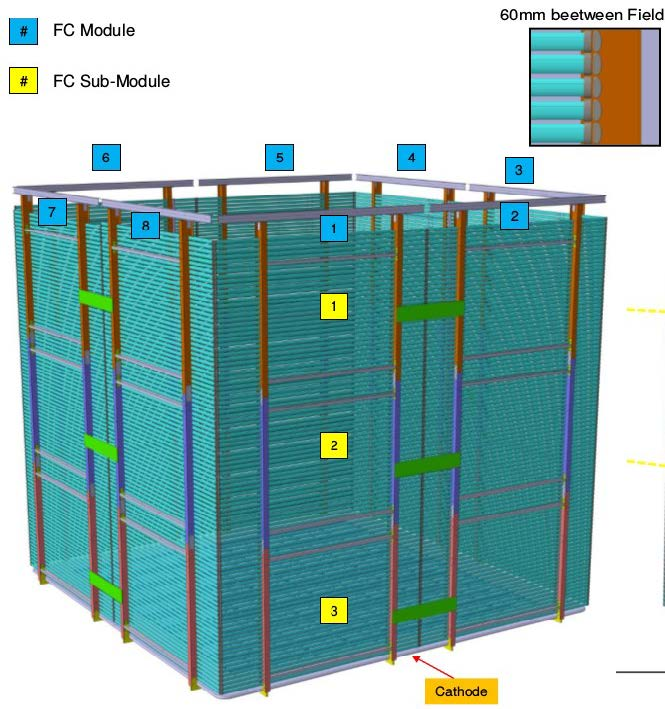
\includegraphics[width=0.35\textwidth]{images/if-dp-fc.jpg}
\caption[]{Conceptual schematic drawing of the field cage assembly for dual phase protoDUNE. Three submodules make up one module, two of which covers $6m\times 6m$ side. }
~\label{fig:if-dp-fc}
\end{figure}

At present, it has been agreed that either CERN or Fermilab will be responsible for purchasing and production of the necessary mechanical parts, including the I--beams that act as the spine of the submodule and the each profile.  The project will purchase the electrical parts: voltage divider boards, resisters and varistors for surge arresting, and the production of electronic boards the field cage. UTA will work in collaboration with the single phase field cage groups (Brookhaven Labs, Stony Brook University, and Louisiana State University) as well as University of Zurich to design the mechanical and electrical components of the dual phase FC. UTA will be responsible for pre-assembly of the submodules, mounting and testing of electrical components, and preliminary testing of as large a field cage sub-module as possible prior to shipping to CERN for installation.

Our postdoctoral researcher, Animesh Chatterjee will be stationed at CERN starting from October 2016 through mid January 2017.  During this period, Chatterjee will work with the ETH and CERN groups to finalize both mechanical and electrical design of the FC for DP protoDUNE and leverage commonality with the SP design as much as possible. The parts for the DP FC will be shipped to UTA for the quality control pre-assembly of submodules, mounting of electrical components, mechanical testing, and low voltage electrical testing. A $6m\times 6m$ electrically independent sub-module will be assembled at UTA and tested at low voltage to ensure electrical functionality. Once the functional testing completes, the submodules will be shipped to CERN for the installation.

The protoDUNE time scale has a hard deadline to complete beam data taking before the LHC shutdown in October 2018.  Therefore, it is essential for our group to contribute early in the process, as outlined in our strategic plan. To meet these goals, Yu plans on staying at CERN bottom half of 2017, utilizing the remaining funds from the agreements with LAPP and ETH to cover the costs for local stay at CERN and the teaching buyout, respectively.  A UTA postdoctoral fellow will also be stationed at CERN together with a graduate student to help with both single and dual phase protoDUNE installation and commissioning.   Yu will then return to the U.S. at the early 2018 at which time Asaadi will be stationed at CERN for the first half of 2018 to continue the effort on the protoDUNE experiments.

We believe this task will help UTA to build up necessary infrastructure for field cage construction in preparation for DUNE and strengthen our position to make essential contribution to the success of DUNE.
